\documentclass[titlepage,danish]{article}

\usepackage{fullpage}
\usepackage[utf8x]{inputenc}
\usepackage[danish]{babel}
\usepackage{color}
\usepackage{amssymb}
\usepackage{amsmath}
\usepackage{fancyhdr}
\usepackage{lastpage}
\usepackage{graphicx}
\usepackage{hyperref}
\usepackage{url}
\usepackage{epstopdf}

\pagestyle{fancy}
\fancyhf{}
\setlength{\headheight}{15pt}
\setlength{\headsep}{25pt}
\lhead{Kursus 02121}
\chead{Space Invaders}
\rhead{s113491, s123692, s123563}
\lfoot{\thepage{} af \pageref{LastPage}}
\rfoot{20/01-2013}

% use when representing code and file names
\newcommand{\code}[1]{\texttt{#1}}

\begin{document}

\title{Space Invaders (kursus 02121)}
\date{20/01-2013}
\author{
  Gadd, Patrick\\
  \texttt{s113491}
  \and
  Veie Færevaag, Markus\\
  \texttt{s123692}
  \and
  Altschuler, Simon\\
  \texttt{s123563}
}
\maketitle

\section{Afgrænsning}
\emph{Her beskrives hvordan afgrænsnings processen foregik og hvad resultatet var.}\\*
Vi vidste fra starten at det er umuligt at vide præcist hvor langt man kan nå i et givent
tidsrum. Derfor var mentaliteten hele tiden at udvikle programmet på så generisk vis som muligt,
således at det ville være nemt at udbygge med nye features, og det uden at koden bliver såkaldt
``slamkode'' (dvs. uorganiseret, dårlig performance, uoverskueligt, etc). Dette er også en af
softwareudviklingens tommelfingerregler: ``It's gonna change''.

Derfor har vi forsøgt at holde koden DRY \footnote{Don't Repeat Yourself:
  \url{http://en.wikipedia.org/wiki/Don't_repeat_yourself}}, velstruktureret og i henhold til velfungerende design principper.

Et par features som vi vidste at vi ville/skulle nå at implementere:
\begin{description}
  \item[Klassisk Space Invaders gameplay] \hfill \\
    Hermed menes ``forsinkede'' skud, bevægende invaders som skyder tilbage, bunkers og den slags.

  \item[Menu system] \hfill \\
    Et system til at vise og styre forskellige skærme (såsom menu, selve spillet, game over,
    highscore), samt et system til at oprette disse på en simpel måde.

  \item[Highscores] \hfill \\
    Et highscore system (som blev implementeret gennem en web service vi også udviklede, således at
    highscoren er global).

\end{description}

Vi brugte de første dage på at udvikle arkitekturen og gennemtænke hvordan tingene skulle
sættes passende sammen. Derefter begyndte vi at udvikle specifikke dele af programmet, og her blev
det også meget nemmere at dele opgaver ud, da delene som regel var fuldstændig uafhængige og dermed
nemt kunne udvikles seperat.

Mere om dette under evaluering (side \pageref{Evaluering})

\section{Features}
\emph{For at give et overblik er der her en liste over de features spillet implementerer}

\begin{itemize}
\item Fem forskellige difficulties, som er gemt i \code{src/model/Configuration.xml}, sådan at man
  nemt kan tune dem og tilføje/fjerne sværhedsgrader
\item Highscores gemt på \url{www.trololo.dk}, sådan at folk på forskellige computere oplever en synkroniseret liste
\item Otte levels gemt i \code{src/model/GameStates.xml}, sådan at man nemt kan tilføje/redigere
  levels.
\item Billeder og lyde, som kaldes gennem \code{SpriteHandler} og \code{SoundHandler}, og ligger gemt i
  \code{resources/}
\item \code{GameElement} og \code{KillableGameElement} som gør det let at tilføje nye objekter til
  spillet
\item Animationer. Vi har lavet et \code{GameElement} kaldet \code{Animation}, så man nemt kan
  tilføje animationer ved at lave et spritesheet og kalde \code{drawAnimation(Graphics g, Animation
    ani)} i \code{GameStateRenderer}. Klassen \code{Animation} indeholder infomation om hvor mange
  frames dets spritesheet indeholder og hvor hurtigt der skal skiftes frame i animationen
\item Farvning af \code{Invaders} alt efter hvor meget liv de har, og om de er "frosne", hhv. rød og blå.
\end{itemize}

\subsection{Gameplay features}Features omkring selve gameplayet:
\begin{itemize}
\item Score: Spilleren får point for at skyde invaders, opsamle gaver samt at gennemføre spillet med
  mere end ét tilbageværende liv.
\item Forskellige typer skud. Man skifter våben på tasterne 1,2 og 3 samt skyder på mellemrum. For
  spilleren:
  \begin{itemize}
  \item 
\includegraphics[scale=0.60]{bullet.eps} Normale: Bevæger sig opad
  \item 
\includegraphics[scale=0.60]{fastBullet.eps} Hurtige: Samme som Normale, men bevæger sig
    dobbelt så hurtigt
  \item 
\includegraphics[scale=0.60]{missile.eps} Missiler: Bevæger sig som Normale, men ved
    kollision med Invader skader de Invaders indenfor et radius på 60 pixels
  \end{itemize} For invaders:
  \begin{itemize}
  \item 
\includegraphics[scale=0.60]{bulletInvader.eps} Normale: Bevæger sig nedad
  \item 
\includegraphics[scale=0.60]{bulletInvaderHoming.eps} "Varmesøgende": Følger spilleren i
    x-aksen, og bevæger sig i y-aksen som Normale. Følger ikke helt naturens love om impuls og
    ændring af denne
  \end{itemize}
\item Forskellige invaders, med forskellige sprites, skudtyper og antal liv (de bliver farvet røde
  alt efter hvor meget liv de har). Invaders kan tilsammen kun skyde én gang pr. tidsenhed. Denne
  ændres ved forskellige sværhedsgrader. Derudover er det kun den forreste invader i en kolonne der kan skyde.
\item En boss, Nicolas Cage, med minions, fuglebure, som svæver rundt om denne. Bossen kan først
  skades når alle dens minions er ødelagt. Modsat invaders, skyder disse minions ved tilfældige
  intervaller, som dog bliver mindre ved højere sværhedsgrader.
\item Bonusser. Hver gang en invader dør, er der en chance for at en bonus spawnes. Skyder spilleren
  disse, går de dog til spilde (vi har valgt ikke at lade invaders kunne skyde dem, da det er meget
  frustrerende for spilleren).
  \begin{itemize}
  \item 
\includegraphics[scale=0.60]{heart.eps} Hjerte (20\% sandsynlighed for at denne spawner):
    Giver spilleren et ekstra liv.
  \item 
\includegraphics[scale=0.60]{snowFlake.eps} Snefnug (40\%): Halverer Invaders hastighed.
  \item 
\includegraphics[scale=0.60]{present2.eps} Gave (40\%): Giver 50 point ganget med
    sværhedsgradens ID (Easy = 1, Trolled =5).
  \end{itemize}
\item Bunkere, der beskytter spilleren, og som kan skydes i mindre stykker af invaders og spilleren.
\item Info-bar i toppen og bunden af skærmen med diverse brugbar information.
\item Reload-bar under spilleren, så man kan se hvornår man atter kan skyde.
\end{itemize}

\section{Implementation}
\emph{Her beskrives spillets strukturelle opbygning, samt vigtige konkrete implementeringsstrategier}
\begin{figure}[h!]
  \centering
  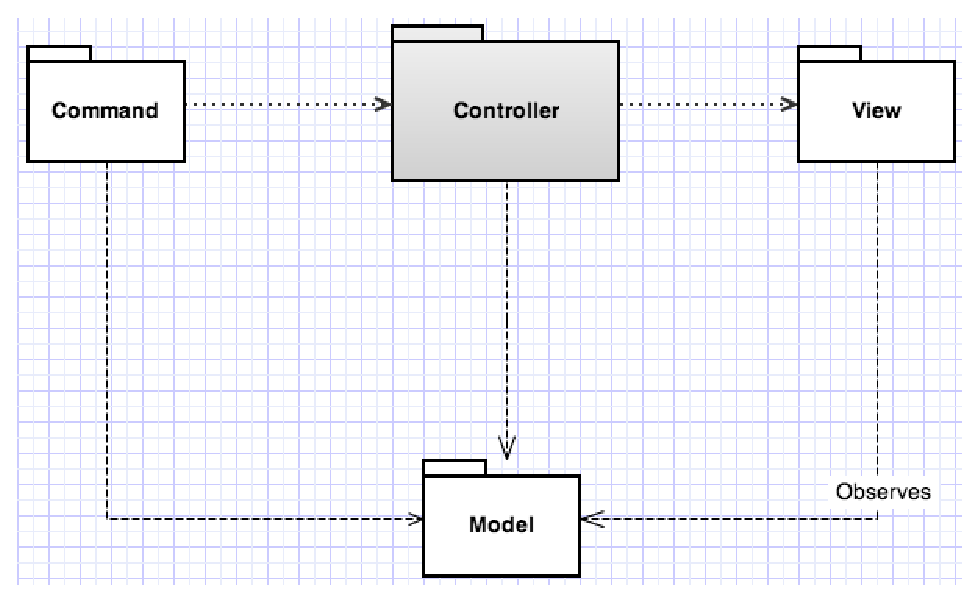
\includegraphics[scale=0.60]{MVC.eps}
  \caption{UML-diagram over spillets overordnede opbygning}
  \label{fig:MVC_diagram}
  \end{figure}
\subsection{Overordnet struktur}
Programmet er opbygget med den klassiske MVC arkitektur som hovedprincip. Det er dog umuligt at definere helt
præcist hvordan en egentlig korrekt implementering ser ud (fordi den ikke findes), men det
overordnede princip gælder mere eller mindre for alle varianter. Disse principper inkluderer
f.eks. at controller ``snakker med'' model og view, og dermed agerer mellemmand mellem de to, samt
at view og model ikke kommunikerer direkte. Sidstenævnte bryder vi en smule, idet vi bruger Observer
pattern.

I vores tilfælde har vi en \code{MainController}, \code{MainView} og \code{MainModel}. Udover det
bruger vi Command pattern til at facilitere eksekvering af ``cachet'' logik, og Observer pattern til
at opdatere views når modellen ændres. Vi gennemgår kort nogle vigtige klasser og principper:

\begin{description}
\item[\code{MainController}] \hfill \\
  Den overordnede controller, som holder instanser af sub-controllers og ikke laver noget egentligt
  arbejde selv. Pointen er, at har man en reference til \code{MainController}, kan man tilgå alle
  andre controllers som getters på denne. Dette gør det nemt og bekvemt at kalde forskellige sub
  controller metoder fra forskellige steder uden at skulle sende hver enkel controller rundt for
  sig.

\item[\code{MainView}]  \hfill \\
  Det øverste view, hvori alle andre views bliver renderet. \code{MainView} indeholder på ethvert
  givent tidspunkt én instans af \code{AbstractViewState}, som bliver renderet i vinduet. Denne
  sættes gennem en Command som kalder en metode på \code{StateController}.

\item[\code{MainModel}]  \hfill \\
  Den overordnede model. Heri ligger al data som beskriver programmets nuværende tilstand. Dette
  inkluderer alt fra hvor stort hovedvinduet er, til hvornår man sidst har affyret et skud. Al data
  som er en del af en specifik spille-session (dvs, hvor mange invaders er der, hvor er de, hvornår
  blev spillet sidst opdateret og renderet), bliver gemt i et \code{GameState} objekt. Dette gemmes
  i \code{MainModel} som det aktive spille-sessions state. Dette objekt er dét som bliver givet til
  en \code{GameController}, der så opdaterer det og sender det til rendering.

\item[\code{Command}s] \hfill \\
  \code{Command}s bliver brugt til at enkapsulere logik der \emph{kan være} afhængig af state. Denne
  logik kan så efterfølgende eksekveres af hvad som helst, når som helst, uden at denne har nogen
  viden om hvad en given \code{Command} \emph{egentlig} gør. Fælles for dem alle er at implementerer
  \code{ICommand} interfacet, hvilket består af en enkelt metode: \code{execute}.  Det er specielt
  bekvemt til f.eks. at eksekvere logik ved tryk på knapper (hvor knappen ikke skal vide hvad den
  laver), men også til generelt at lagre og udføre logik fra andre steder.  Vi har udvidet det klassiske
  command pattern en smule ved at implementere en \code{chain} metode, som effektivt sætter
  \code{Command}s sammen som en linked list (ikke cirkulær) og returnerer en ny command.

\item[Observers] \hfill \\
  \code{MainModel} implementerer Java's \code{Observable}. Det er en måde for et objekt at eksponere
  et interface som gør et andet objekt, en \code{Observer}, opmærksom på hvornår den er
  opdateret. Vha. observer pattern gøres dette fuldstændig decoupled, og \code{MainModel} har altså
  ingen viden om hvem der lytter efter dens ændringer. Ændringerne annonceres gennem
  \code{Oberservable}s \code{notifyObservers} metode.
\end{description}

Vi har valgt ikke at udvikle tests til projektet. Vi kunne have lavet en masse Unit Tests som kunne
have fanget fejl for os, eller endda udviklet i TDD stil. Vi vurderede dog at til et projekt af
denne størrelse og art at det ikke ville være det værd. I stedet har vi været grundige for at
udvikle i en stil der forebygger fejl og testet manuelt løbende.

\subsection{GameController}
Står primært for at opdatere \code{GameState} samt at få \code{GameStateRenderer} (kaldet \code{renderer}
under \code{GameController}) til at rendere \code{GameState}. Derudover anvendes en
\code{javax.swing.Timer} som spillets opdaterings mekanisme. Timeren eksekverer en
\code{UpdateGameStateCommand} ved hver trigger.

Metoden \code{updateGameState()} gør følgende (i kronologisk rækkefølge):
\begin{enumerate}

\item \code{currentTime} bruges til at udregne \code{timeDelta}, gemmes i det aktuelle
  \code{GameSate} så man kan se hvornår det sidst blev opdateret, samt til at afgøre om
  \code{Player} og \code{Invaders} må skyde i denne update.

\code{timeDelta} bruges til at bevæge samtlige \code{GameElement}’er afhængigt af den tid der er
gået, sådan at de for spilleren bevæger sig med konstant hastighed uafhængigt af om tiden mellem
updates varierer.

\item Kontrollerer om \code{GameStateState} er \code{Running}/\code{Waiting}/\code{Paused}. Hvis
denne enum er \code{Waiting}/\code{Paused} returnerer metoden og kører dermed ikke videre. Hvis den
er \code{Running} fortsætter den og tjekker om spilleren eventuelt trykker ESC for at pause (og returnere).

\item Herefter bliver alle \code{GameElement}’erne opdateret. Dette indebærer at:
\begin{itemize}
\item der bliver tjekket med \code{utils.Input} om en listener er aktiveret af spilleren
\item der vha. \code{controller.gamestatehandler} bliver rykket relevante elementer, oprettet skud og kontrolleret for kollisioner
\item der endeligt fjerne de elementer der er blevet mærket som ``destroyed'' med metoden \code{sweep()}
\end{itemize}


\item Tjekker om man har vundet/tabt og kalder en \code{Command} hvis dette er tilfældet. Kalder
\code{GameStateRenderer.render()} og renderer hermed det aktuelle \code{GameState}.

\item Kalder \code{GameStateRenderer} og får denne til at rendere det aktuelle \code{GameState}. Vi
burde teoretisk set have haft en overordnet klasse som kaldte \code{updateGameState()} og
\code{GameStateRenderer.render()} uafhængigt af hinanden, sådan at \code{GameState} kunne opdateres
uden at nødvendigvis blive renderet, i tilfælde af at det skulle blive nødvendigt.

\item Slutteligt opdateres tiden gemt i \code{GameState}.
\end{enumerate}


\subsection{utils.Mathx} Indeholder belejlige matematiske metoder, hvoraf den eneste rigtigt
interessante er \code{circleRectangleIntersects()}, som er noget mere advanceret end detektion
mellem rektangel-rektangel eller cirkel-cirkel. Den ser således ud:

\begin{verbatim}
boolean circleRectangleIntersects(GameElement rect, Coordinate circ, double radius){

  double rectCenterX = rect.getPosition().x + ((double) rect.getWidth()/2);
  double rectCenterY = rect.getPosition().y + ((double) rect.getHeight()/2);

  double circleDistanceX = Math.abs(rectCenterX-circ.x);
  double circleDistanceY = Math.abs(rectCenterY-circ.y);

  if (circleDistanceX > (rect.getWidth()/2 + radius)) { return false; }
  if (circleDistanceY > (rect.getHeight()/2 + radius)) { return false; }
}
\end{verbatim}

De to ovenstående \code{if} conditionals har udelukket alle tilfælde hvor cirklen ligger udenfor en
forstørret udgave af rektanglen (rektanglen + radius). Dette svarer til det lyserøde område, som strækker sig uendeligt i retningerne væk fra rektanglen, på
figur \ref{fig:col_rect}.

\begin{figure}[h!]
  \centering
  
\includegraphics[scale=0.60]{rekt_cirk_02.eps}
  \caption{Farverne repræsenterer de forskellige tjek som bliver udført i funktionen \code{circleRectangleIntersects()}}
  \label{fig:col_rect}
\end{figure}

Derfor vil cirklen ligge indenfor rektanglen+(cirklens radius) for de to nedenstående \code{if}
conditionals. Disse to tjekker om cirklens centrum ligger i de på illustrationen lysegrønne områder,
eller ligefrem indenfor rektanglen (mørkegrå).
\begin{verbatim}
    if (circleDistanceX <= (rect.getWidth()/2)) { return true; } 
    if (circleDistanceY <= (rect.getHeight()/2)) { return true; }
\end{verbatim}	    
Tilbage er der kun at kontrollere hjørnerne af den forstørrede rektangel (kvadrater med cirklens
radius som sidelængde). Dette svarer til de hvide områder på figur \ref{fig:col_rect}.
\code{cornerDistanceSquared} er cirklens centrums afstand til den oprindelige rektangels hjørner
kvadreret.
\begin{verbatim}
    double cornerDistanceSquared = Math.pow((circleDistanceX - rect.getWidth()/2),2) + 
        Math.pow((circleDistanceY - rect.getHeight()/2), 2);
    return (cornerDistanceSquared <= Math.pow(radius,2));
}
\end{verbatim}
Er cirklens centrum længere væk end dens radius er der ikke kollision.


\subsection{service.HighscoreService}

Indeholder metoder som kan gemme og hente highscores i en XML-fil vha. vores webtjeneste, på domænet \url{http://trololo.dk}.

For at gemme, kalder metoden en url med almindelige GET-parametre med informationerne spillernavn, score og sværhedsgrad. Blandt disse parametre er der også en \emph{token}, som fungerer som en primitiv sikkerhed i form af en "hemmelig" \code{String}. Denne token bliver hentet via den frit tilgængelige \code{Configurations.xml}. Umiddelbart burde vi have hardcodet token ind i koden, sådan at den ikke kan aflæses direkte. Da vi har brugt Git til versionskontrol, ligger koden dog frit tilgængelig. Derudover kan man også sniffe web trafik, og dermed aflæse token. Som kontrol får man en streng retur, som fortæller om alt gik vel eller om noget gik galt.

At hente highscores fungerer efter samme princip, med en (valgfri) \emph{limit} parameter, som angiver antallet af scores som skal returneres.

Lokalt bliver de behandlet af \code{HighscoreController}, som objekter af klassen \code{HighscoreEntry} (\code{model}). \code{HighscoreEntry} indeholder naturligvis nødvendig information, samt implementerer \code{Comparator} og \code{Comparable}, sådan at kontrolleren nemt kan sortere efter score.

Webservicen er udviklet i Python med Django\footnote{Django: \url{https://www.djangoproject.com}} web frameworket.

\subsection{Ressourcebehandling (\code{service.resources})}
Indeholder \code{SpriteHandler} og \code{SoundHandler} som behandler vores lyde og billeder af klasserne \code{Sound} og \code{Sprite}. Pointen med disse klasser er at have en centraliseret tjeneste som henter lyd og billeder, og cacher disse i et \code{HashMap}\ for at spare ressourcer. For at sikre at de ikke bliver cachet flere gange, er klassen lavet som en singleton (den kan kun have én instans).

\subsection{XML-parsing (\code{service.parsing})}
Som XML-parser bruger vi \code{SAXParser} som ligger i \code{javax.xml.parsers}. Vores instans af SAX-parseren får en XML-fil og en handler, som ligger i den angivne mappe. Handleren extender \code{DefaultHandler}, og overrider metoder som f.eks. \code{startElement()}. Her kan vi definere hvad som skal ske når den får et instans af hvert element i en XML-fil, som f.eks. et \code{\textless highscore name ="Ola Normann" score="1337" \textgreater}. Dette specifikke element vil blive gemt i en ny \code{HighscoreEntry} i et array som så kan hentes af en Controller.

\subsection{Collision detection}
Dette er en essentiel del af spillet, og derfor er det vigtigt at det fungerer optimalt. Vi har brugt en diskret tilgang \footnote{\url{http://en.wikipedia.org/wiki/Collision_detection\#A_posteriori_.28discrete.29_versus_a_priori_.28continuous.29}} til at opfange kollisioner mellem objekter i spillet, da dette er yderst simpelt at implementere. Vi tjekker hvert objekt med samtlige potentielt relevante\footnote{Relevante i den forstand at det giver mening at tjekke for kollision. Eksempelvis tjekkes der ikke for kollision mellem bunkers og player} objekter, hvilket formodentligt er noget ineffektivt.

Derudover er der mulighed for at en kollision ikke bliver opfanget. Dog har vi sat frameraten så højt (ca. 160 FPS), at spillets hurtigst bevægende objekt, "fast bullet", ikke kan nå helt igennemt spillets mindste, "bunker part", på en enkelt frame. Dette ses da  "fast bullet" bevæger sig 3/4 pixels * timeDelta, og højden af en "bunker part" er 12 pixels, hvilket vil kræve at timeDelta er mindst 16 millisekunder. Vi kapper kunstigt timeDelta til maks. 15 millisekunder. Vi mener nemlig at det er rimeligt, og for at eftervise det lavede vi tre tests på et minut hver:

\begin{center}
    \begin{tabular}{ | l | l |}
    \hline
    Frames & timeDelta \textgreater= 16  \\ \hline
    9872 & 29 \\ \hline
    9758 & 24  \\ \hline
    9975 & 37  \\
    \hline
    \end{tabular}
\end{center}

Da timeDelta i gennemsnit bliver cappet én gang for hver gang der er vist 330 frames, mener vi bestemt det er en acceptabel løsning.
Havde det været et problem, ville en mulig løsning på problemet være, at køre \code{updateGameState()} flere gange pr. frame, sådan at den blev kørt n gange med \code{timeDelta} delt med n (og fornuftig afrunding, da det er et heltal). Dette ville naturligvis dog kræve yderlig regnekraft.

\section{Evaluering} \label{Evaluering}
\emph{Vi evaluerer proces og resultat af arbejdet.}
\subsection{Proces}
Vores udviklingsproces viste sig at fungere godt. Versionsstyring er guld værd, og den eneste
ulempe vi fandt ved Git er, at det kan betale sig at holde styr på hvem der arbejder hvor, for at
undgå for meget merging arbejde.

Lige i starten var alle med til sammen at udtænke den overordnede opbygning, men som fundamentet
efterhånden blev lagt, kunne vi dele arbejdet op i isolerede opgaver som man individuelt fik ansvar
for at implementere. Denne fremgangsmåde virkede godt, og var meget effektiv, både fordi det var
nemt at projektstyre, og fordi vi hver især fik lyst til at levere et godt stykke arbejde.

Samarbejdet har været godt, alle har arbejdet lige, og har sat deres præg på resultatet. Alle har været
gode til at sætte sig ind i, og respektere andres arbejde.

\subsection{Kommentering \& Javadoc}
Vi har i høj grad kommenteret og forsøgt at give alt logiske navne, sådan at det vil være nemmere at arbejde videre på projektet selv efter en lang pause - eller for andre at sætte sig ind i det. Der er genereret et Javadoc i form af en samling HTML-dokumenter under spaced/doc/

\subsection{Samlet resultat}
Vi er meget tilfredse med hvordan resultatet blev. Det gik hurtigere og hurtigere at få
implementeret nye features, i takt med at vi vænnede os til strukturen, og den viste sig at holde
til de udvidelser vi havde i sinde.

Det betalte sig på alle måder at lave spillet generisk nok til at det ikke var designet med et helt
konkret feature sæt i sinde. Det har været nemt og bekvemt at udvikle forskellige dele af spillet
samtidig, også selvom vi har pushet og pullet ofte - 238 commits i skrivende stund! 

Vi har gennem hele projektet brugt pixels som måleenhed til afstande. I virkeligheden er dette ikke
en god ide, fordi det ikke er skalerbart. I stedet bør man bruge en defineret afstandsberegning,
f.eks. ``meter'', som man så via en hjælpemetode regner om til pixels. På den måde bliver alle
afstande både skalérbare og man kan hurtigt ændre sine afstandsforhold. Ydermere er det nemmere at
forestille sig, da man kan tænke álá ``Skibet skal være 2 meter'' bredt, i stedet for ``Skibet skal
være 60 pixels'' bredt.

\subsection{Videre udvikling}
En ting vi burde lære at blive bedre til er at rebase og håndtere commits, for vi endte ofte med
at pushe 5 commits ad gangen, hvoraf de 4 var merge commits af branches og conflict
resolutions. Vores hoved repository endte op med alt for mange commits, så det ville være svært, i
nogle tilfælde, at snævre en feature ned til et bestemt commit i timelinen.

Hvis vi skulle arbejde videre med projektet ville næste skridt være at strømline al kode, og
derefter lave tests, for at sikre stabilitet.

\section{Værktøjer}
\emph{Kort gennemgang af de værktøjer vi har brugt}
\subsection{Versionsstyring}
Til projektet har vi brugt Git\footnote{Git: \url{http://git-scm.com}}. Det har visse fordele over
f.eks. SVN og Mercurial (og specielt TFS). Kort opsummering af grunde til at bruge Git:

\begin{description}
  \item[Distribueret] \hfill \\
    Git er en af de eneste fuldstændig distribuerede VCS'er. Man arbejder altid i sit eget lokale
    repository, og kan gøre hvad man vil, uafhængigt af alle andre. Man har så et hostet
    \emph{main} repository, som regel kaldet origin, som vi hoster på GitHub \footnote{GitHub:
      \url{http://github.com}}. 

    En fremragende følge af dette er at alle kan arbejde uden netforbindelse, og da et commit bliver
    committet lokalt går det \emph{meget} hurtigere, da der ikke skal forbindes til server.

  \item[Branching] \hfill \\
    Branching er meget mere ligetil i Git i forhold til SVN og Mercurial, og skift af branch samt
    merge af disse er intuitivt og nemt.

  \item[Performance og størrelse] \hfill \\
    Git er utroligt hurtigt, og utrolig god til at kompresse data (til sammenligning fylder Mozillas
    samlede repo med commit historie 12gb i SVN og noget ala 400mb i Git!).
\end{description}

\subsection{IDE}
Som IDE har vi brugt både Eclipse\footnote{Eclipse:\url{http://www.eclipse.org}} og
NetBeans\footnote{NetBeans: \url{http://www.netbeans.org}}. De to minder meget om hinanden, er begge
open source og valget er en smagssag. Begge har de også integration af versionsstyring, hvor vi dog
har holdt os til command-line Git, da den slags GUI værktøjer som regel er lidt ustabile.

\subsection{Diverse}
Vi har brugt Paint.NET\footnote{Paint.NET: \url{http://www.getpaint.net}} til at redigere grafik, og
Audacity til lydredigering\footnote{Audacity: \url{http://audacity.sourceforge.net}}.

\end{document}